\chapter{Kinect Analysis}
\graphicspath{{./KinectData/img/}}

As mentioned in the introduction, a closer look to the Kinects data characteristics is taken
within this document to be able to implement a sign detection method. 
For this work the Kinect RAW fromat was used, each value has 16 bit and shows the
depth for the pixel in millimeters. A depth of zero means that no valid data is available for
this pixel.

\section{Surface Problems}
There are a few cases when the Kinect is not able to deliver any depth data from a surface.

First of all, it does not work with translucent materials like glass. The projected
points are just diffracted away, when they hit in a small angle (see figure \vref{figure:glas}). 
It's possible to look through a translucent surface, but only if it's clear and the angle from the 
camera to the surface is not to big.
\begin{figure}[htp]
\begin{center}
  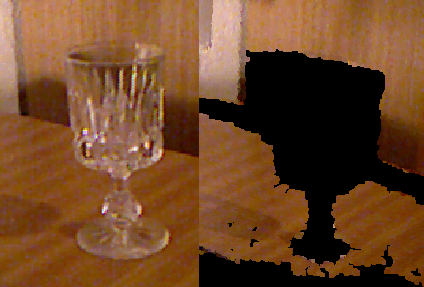
\includegraphics[height=\textheight/3]{glas.png} 
  \caption{Glass (Webcam/Pointcloud)}
  \label{figure:glas}
\end{center}
\end{figure}
 
Another problem are mirrors. Mirrors will also diffract the IR spots away, 
so it's not possible to get any depth data from their surfaces (see figure \vref{figure:mirror}).
\begin{figure}[htp]
\begin{center}
  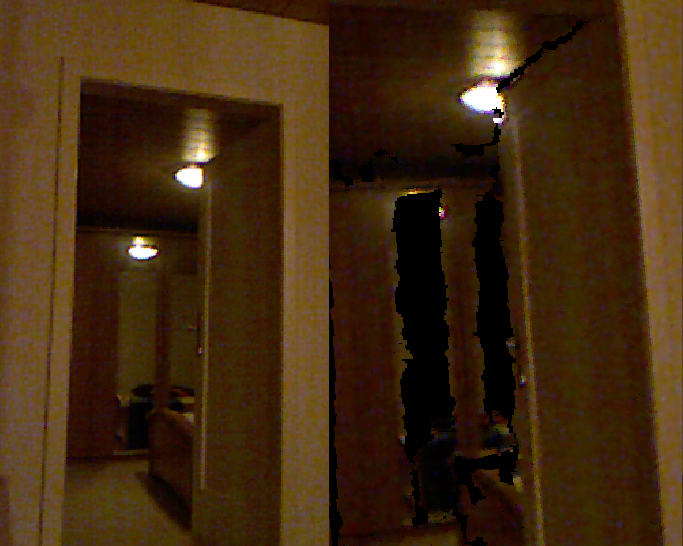
\includegraphics[height=\textheight/3]{Mirror.png}
  \caption{Mirror (Webcam/Pointcloud)}
  \label{figure:mirror}
\end{center}
\end{figure}

If the sun lights up a surface directly, it will outshine the IR-spots so this will blank out the surface
in the resulting depth image too (see figure \vref{figure:sun}).
\begin{figure}[htp]
\begin{center}
  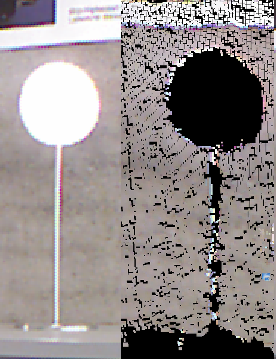
\includegraphics[scale=1.2]{Sun.png}
  \caption{Sunlight on a surface (Webcam/Pointcloud)}
  \label{figure:sun}
\end{center}
\end{figure}

On surfaces which are too close to the camera, the IR-spots will melt together preventing the camera from
identifying their location (see figure \vref{figure:close}), which leads to the same result as in the previous cases.
\begin{figure}[htp]
\begin{center}
  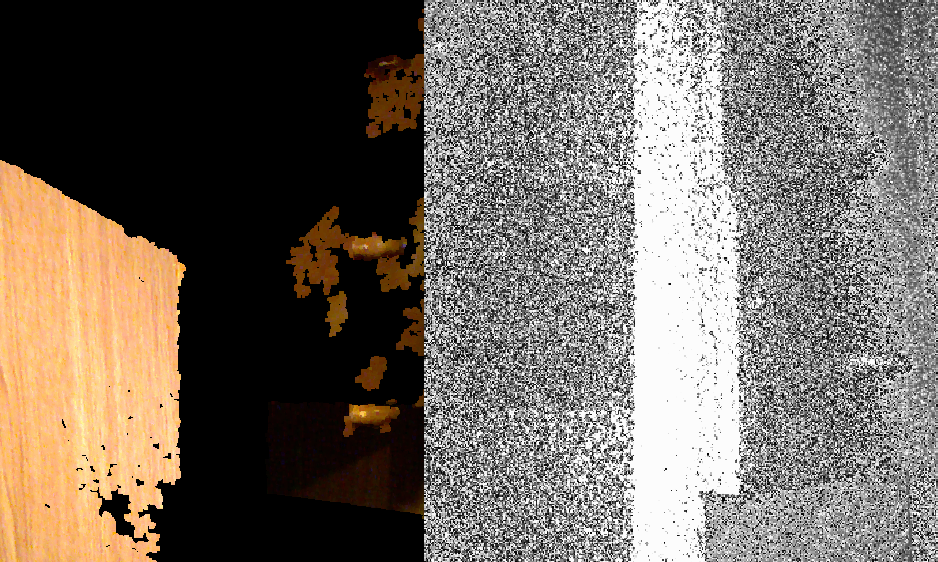
\includegraphics[scale=0.7]{ToClose.png} 
  \caption{Kinect to Close to a Surface (IR sensor/Pointcloud)}
  \label{figure:close}
\end{center}
\end{figure}
\clearpage 
 
\section{Analyzing Tools} 
While this work, multiple analyzing tools have been created. Those were created as
nodes to easily connect with the OpenNi driver package in the ROS system.
\subsection{DepthImageAnalyzer}
In the beginning a Qt-GUI node was created to get in touch with the depth images and 
their values and how they look like. It is able to show a depth image in the double
format and if the user clicks into the picture it will show the corresponding 
value of the pixel. It also allows to set a depth range to highlight. 
Figure \vref{figure:DIA} shows the GUI of this node with a highlighted depth range.

\begin{figure}[h!tp]
\begin{center}
  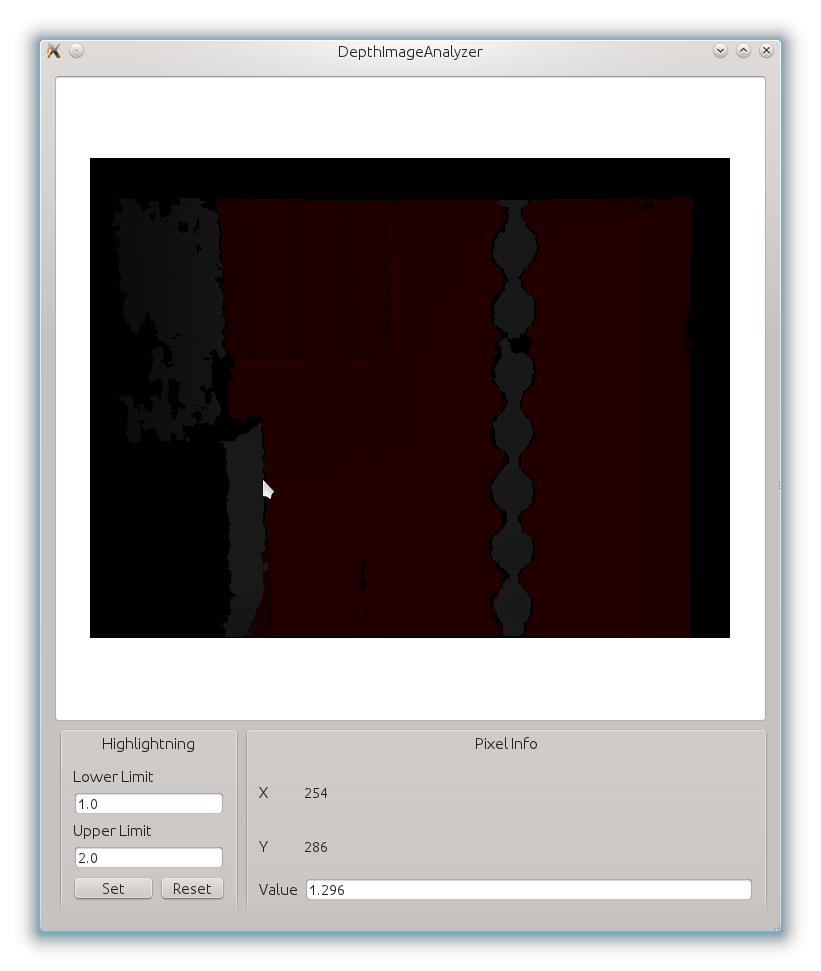
\includegraphics[width=\textwidth]{DepthImageAnalyzer.jpg}
  \caption{DepthImageAnalyzer GUI}
  \label{figure:DIA}
\end{center}
\end{figure}
\clearpage 


In the later process of this work it was not needed anymore, because showing the point cloud
in rViz showed to be more effective in analyzing data and debugging applications.

\subsection{PointCloud creation with custom topics}
A 3D display of the point cloud is very useful for debuging and filtering techniques, it directly shows what 
happens to the data, when a special filter is applied.
To create point cloud messages for other topics than those from the Kinect node, it is necessary to
create specific launch files. Launch files are xml-files which are used to start multiple nodes (applications) 
in one go with the roslaunch tool from ROS. 


\begin{lstlisting}[caption={Standalone Point Cloud}\label{lst:stal_pcl},language=xml]
<node pkg="nodelet" type="nodelet" name="PointCloudAdvisor" 
 args="manager" output="screen"/>

<node pkg="nodelet" type="nodelet" name="points_xyzrgb_Advisor" 
	args="load depth_image_proc/point_cloud_xyzrgb PointCloudAdvisor --no-bond">
    <remap from="rgb/image_rect_color"        to="/signDetection/out_rgb" />
    <remap from="rgb/camera_info"             to="/signDetection/camera_info" />
    <remap from="depth_registered/image_rect" to="/signDetection/out_depth" />
    <remap from="depth_registered/points"     to="debug_cloud" />
</node>
\end{lstlisting}

As seen in the listing for creating a point cloud from different topics a nodelet manager and a 
depth\_image\_proc/point\_cloud\_xyzrgb nodlet is needed. Inside the node tag of the nodelet
there are the remapping tags, to connect the nodelet with the custom topics.


\subsection{Tool for various data fetching and filter testing}
The tool was named disturbance\_filter\_calculator, the name is still reminding what it was intended to do in the first place
. It should filter out the noise by creating a picture of it on a flat surface. This didn't work because of the special 
autoranging feature of the Kinect which will be discussed later. Currently the Tool can be used to fetch data points or to
draw a pattern of lines in the RGB image which is mapped over the point cloud. It also can tell the users which data points
are in a given distance and which not, by painting the pixels of the RGB image green for being in the specified distance
and red if not. This feature helped to realize about the missing values which are also discussed later. It also includes
some of the first tries to filter and blur the depth image, but as the project advanced it was decided to move the 
filter code to a new clean node in a new package to save compiling time, leaving the disturbance\_filter\_calculator 
node as it was. A screenshot of the robot visualizer displaying the point cloud with a few points in the specified distance
can be seen in figure \vref{figure:distFilCal}.

\begin{figure}[htp]
\begin{center}
  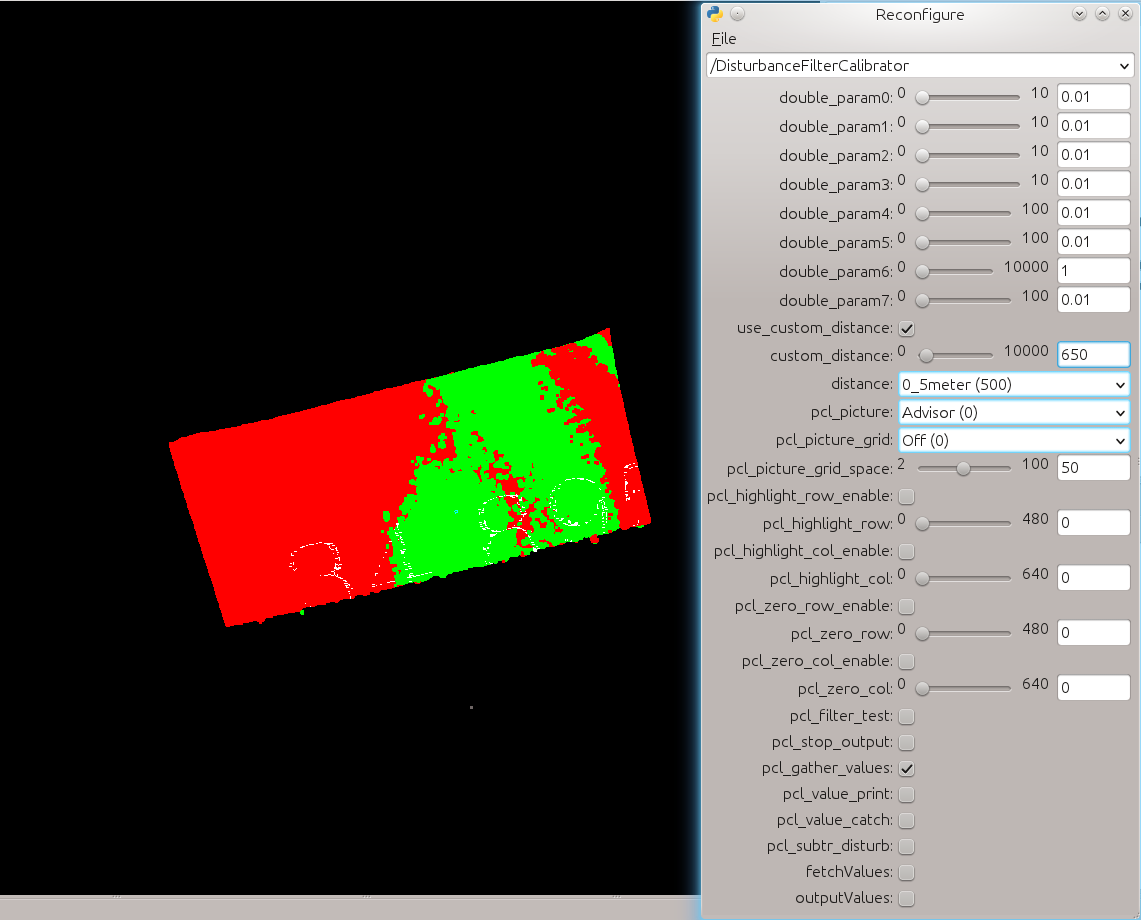
\includegraphics[width=\textwidth]{disturbanceFilterCalibrator.png}
  \caption{disturbance\_filter\_calibrator: rviz and reconfigure\_gui}
  \label{figure:distFilCal}
\end{center}
\end{figure}


\section{Disturbances}
While pointing the Kinect to a flat surface the noise fractals (see in figure \vref{figure:noise}) 
seem to reappear at the same position. So it was decided to try to remove them with capturing a single image 
from a flat surface and subtract the current distance to get a picture which can be substracted from further collected
frames to remove the noise. This was a nice idea but it didn't work as expected. 
There are some special vertical fractals (see in figure \vref{figure:verticals}) 
inside the image which seem to be the result from an autoranging feature of the camera, those fractals
always create one data step in the picture. The biggest problem is that the structure of the noise fractals
in figure \vref{figure:noise} changes with their appearance and their number. 
The number of those vertical lines ranges from 0 to a spotted maximum of 9. 
They do always appear on a special range, seem to be symetrical or 
nearly symetrical to the center and their number is never even but they are not fixed to a special column of pixels. 
\begin{figure}[htp]
\begin{center}
  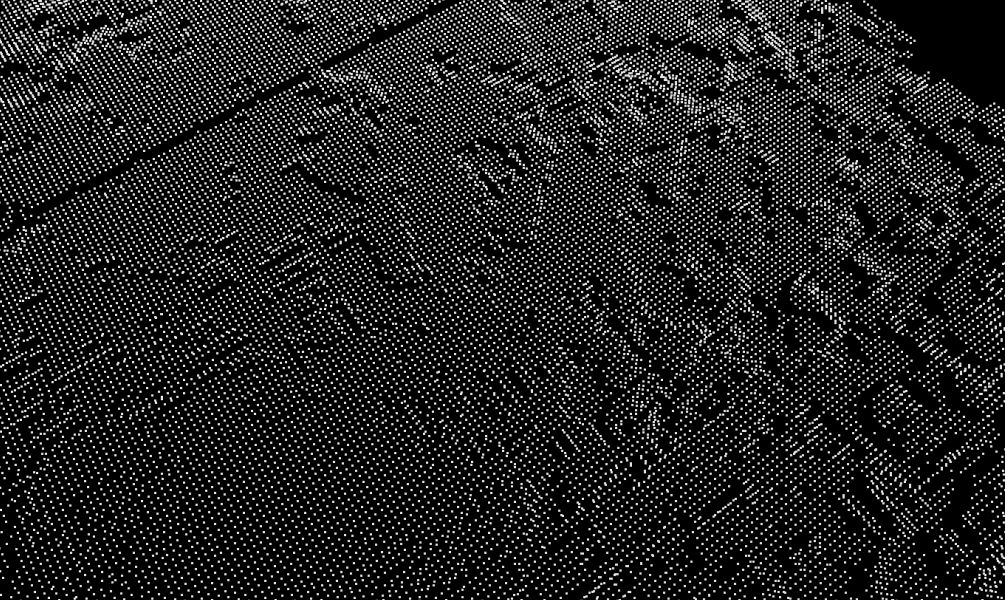
\includegraphics[width=\textwidth]{noise.png}
  \caption{Noise (Pointcloud)}
  \label{figure:noise}
\end{center}
\end{figure}

\begin{figure}[htp]
\begin{center}
  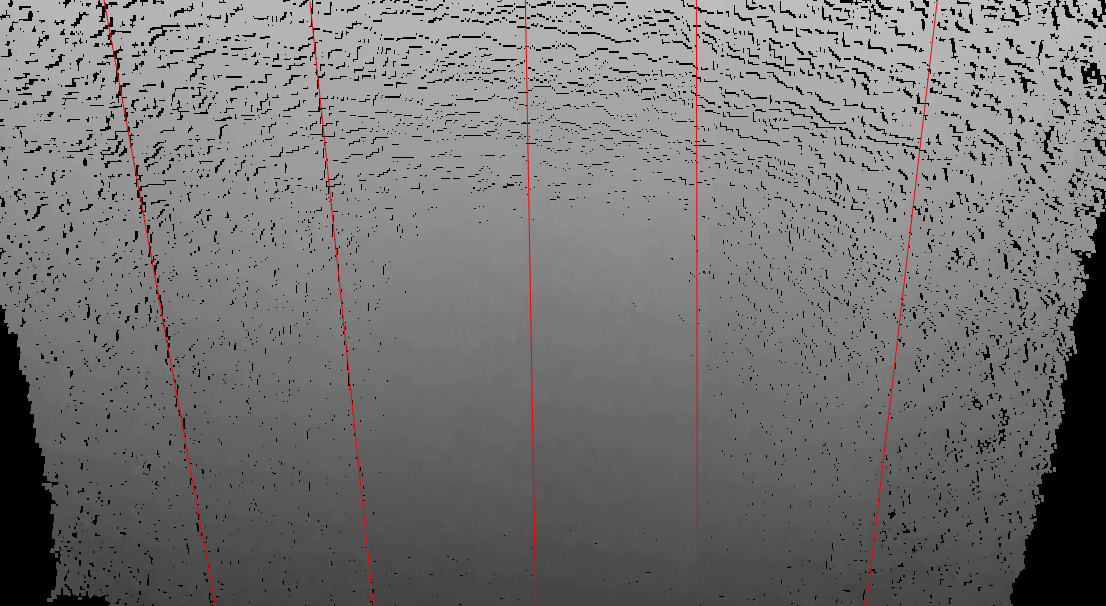
\includegraphics[width=\textwidth]{verticalFractals.png}
  \caption{Vertical Fractals (Pointcloud)}
  \label{figure:verticals}
\end{center}
\end{figure}

\section{Resolution Depending the Depth} \label{resdepDepth}
When creating the diagram in figure \vref{figure:LaserKinect}, which shows the occuring values from the camera 
at a specific distance from a plain and parallel surface and the distance measured with a laser distance measurement 
device(see in figure \vref{figure:hilti}),it was realized, that many values just do not exist. The camera never outputs 
these values. After realizing this fact, it was decided to look for the available values, their number and the values which 
never occur.The figures \vref{figure:depths1} and \vref{figure:depths2} show the distance on the left, 
the available values (black) and not availabe values (white) in the middle and the number of the missing values between them 
on the right. Figure \vref{figure:DepthValueDiff} shows the number of missing values in relation to the depth.

\begin{figure}[htp]
\begin{center}
  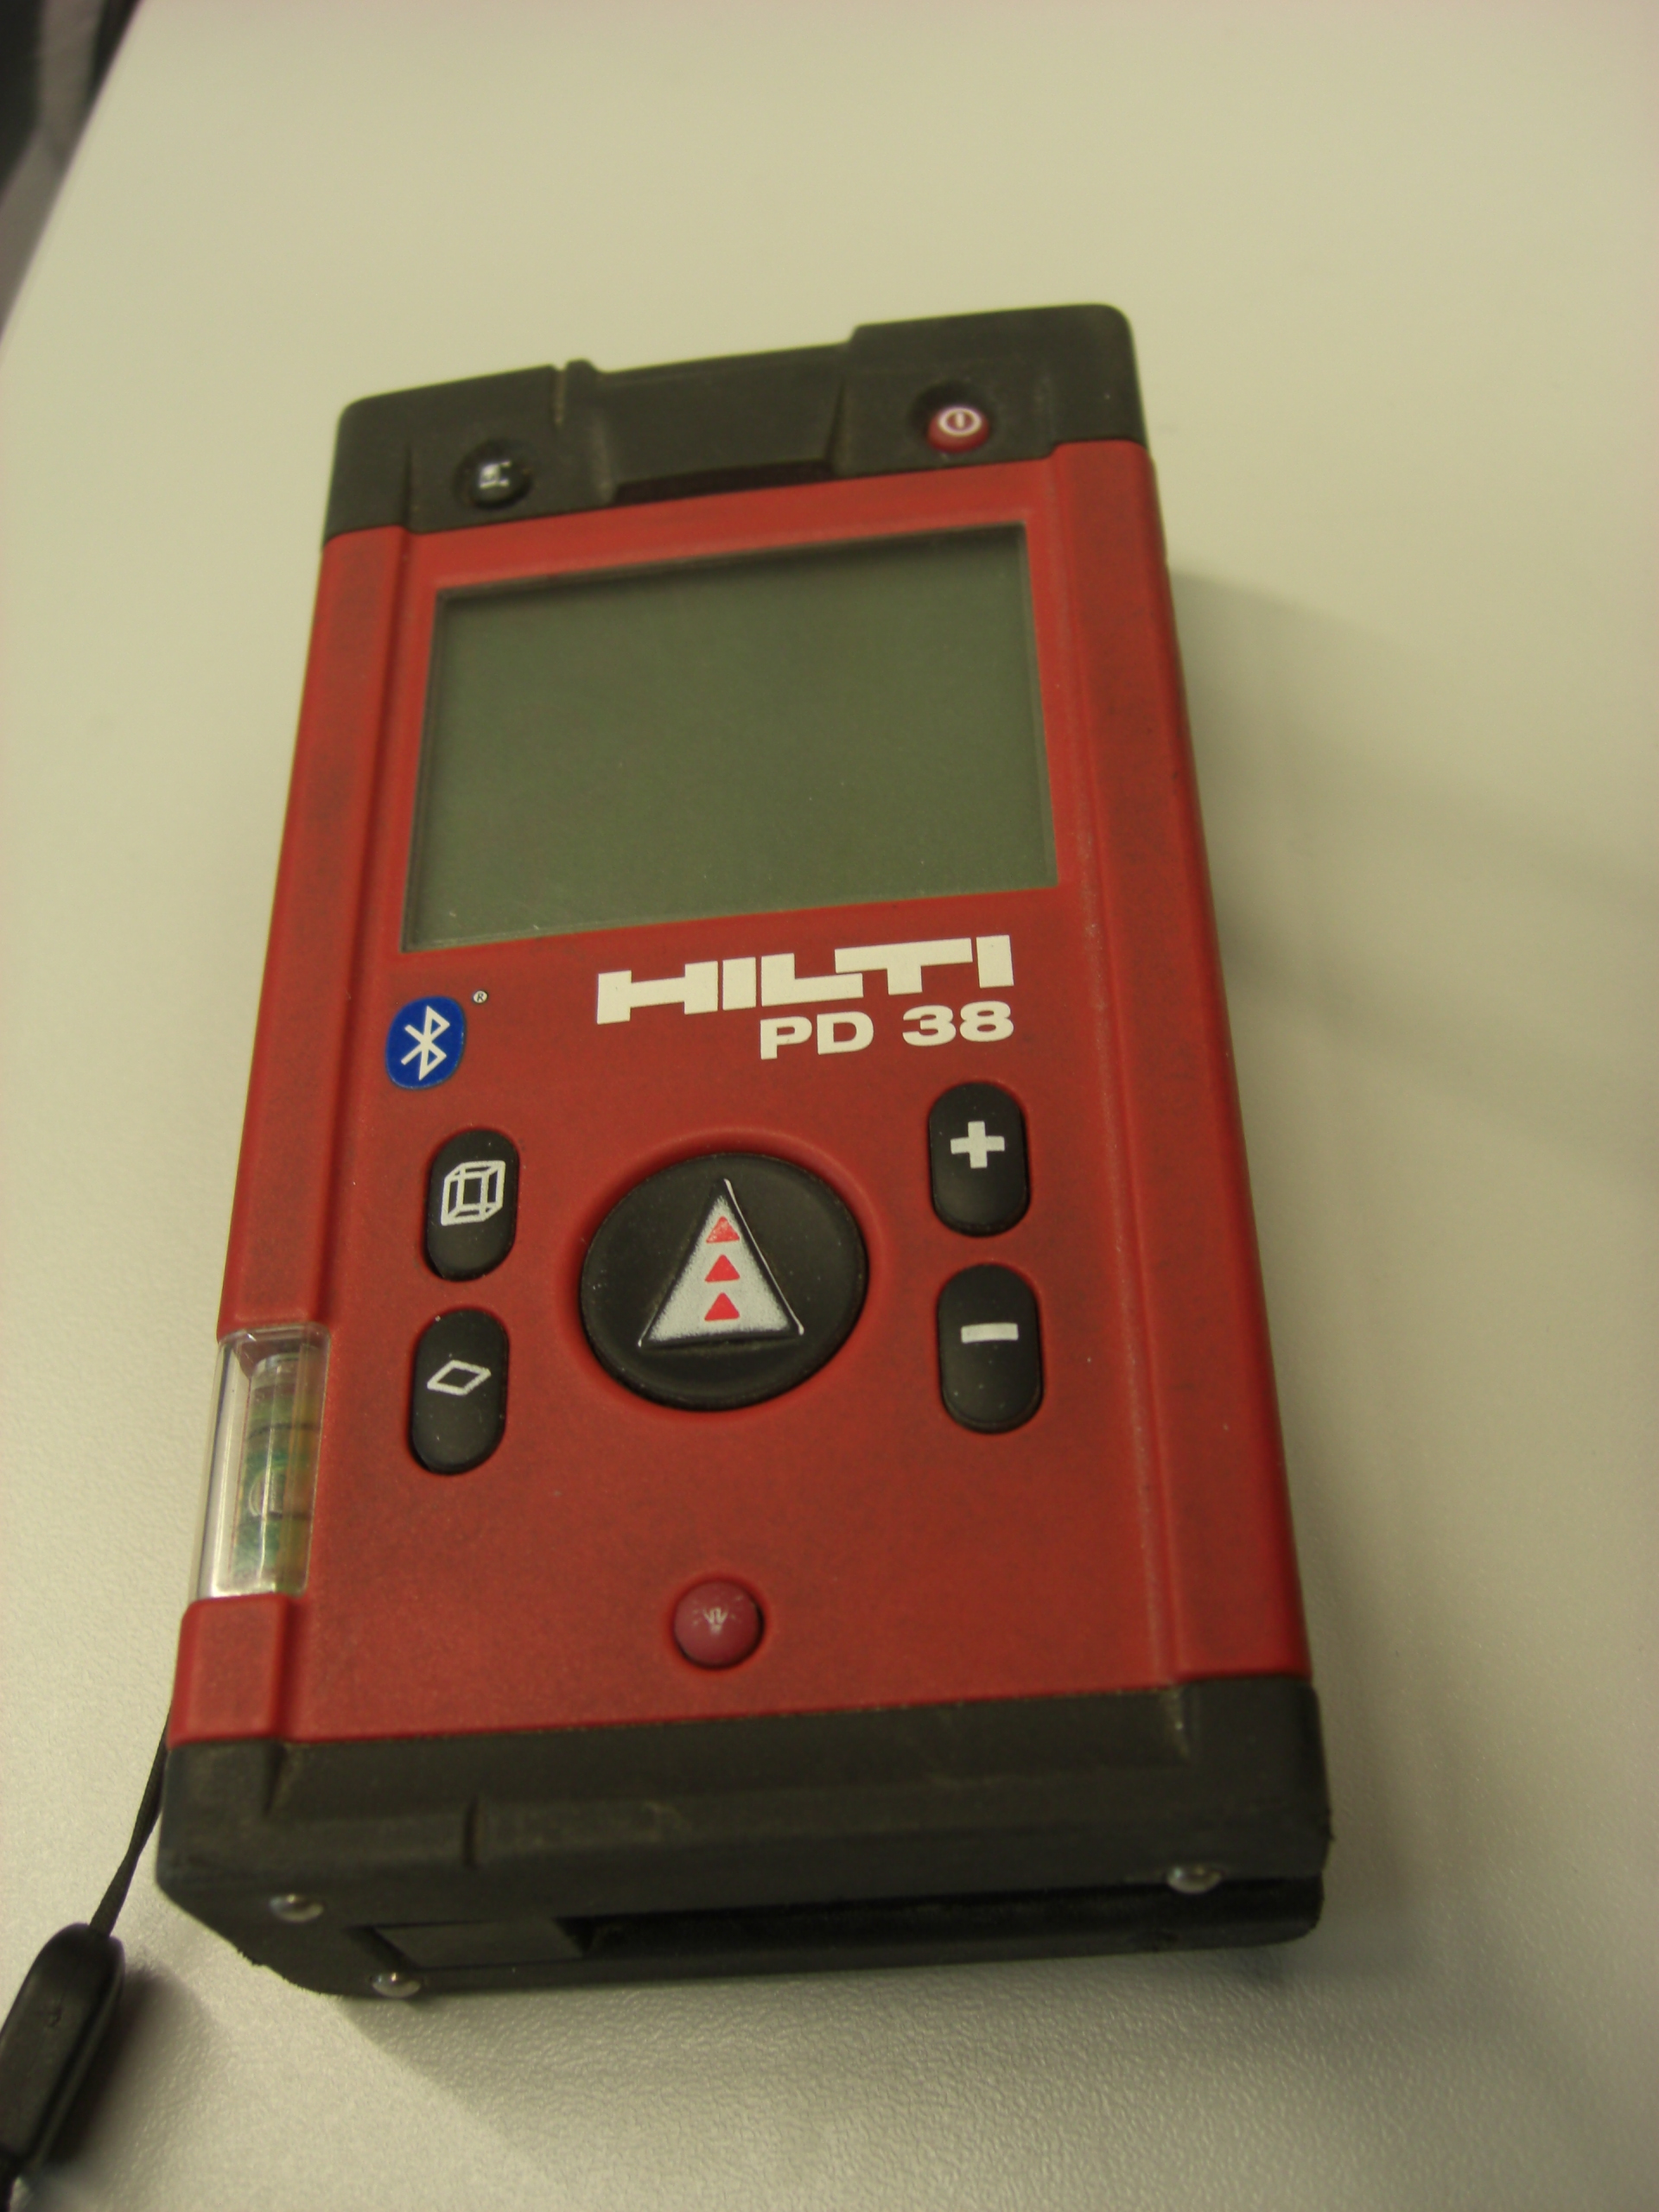
\includegraphics[width=\textwidth/4]{hiltipd38.jpg}
  \caption{Hilti PD38 Laser Distance Measurement Device}
  \label{figure:hilti}
\end{center}
\end{figure}
\begin{figure}[htp]

\begin{center}
  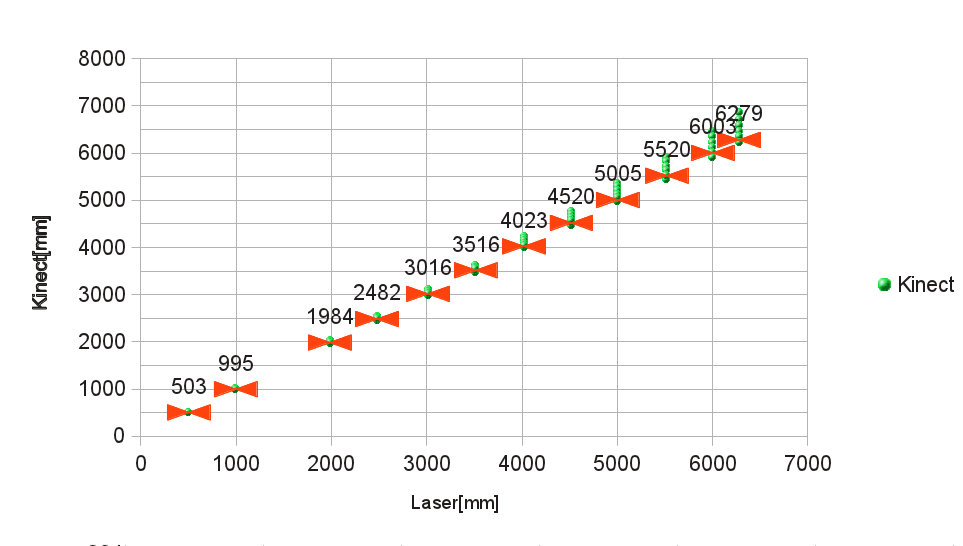
\includegraphics[scale=0.8]{LaserDistanceKinectDistance.png}
  \caption{Distance measured by Laser and by Kinect}
  \label{figure:LaserKinect}
\end{center}
\end{figure}

\begin{figure}[htp]
\begin{center}
  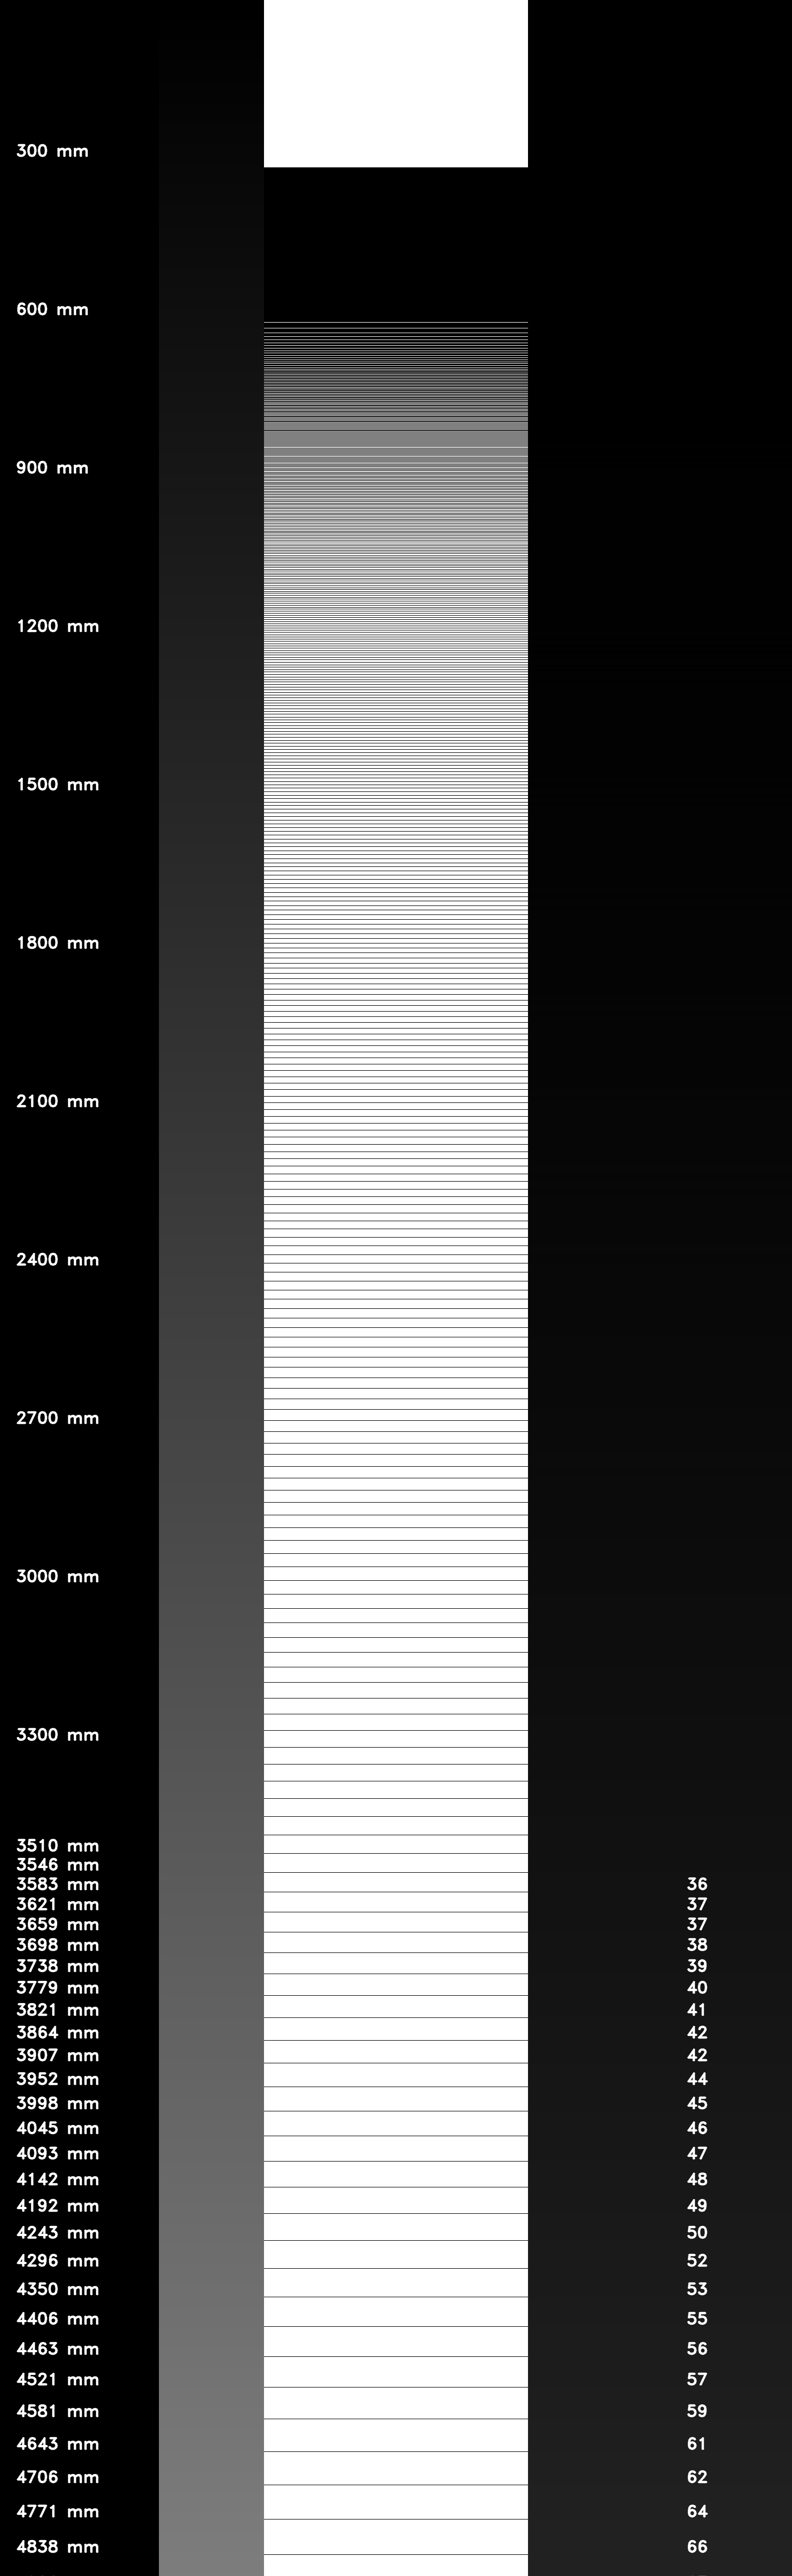
\includegraphics[scale=0.1]{availdepths0.png}
  \caption{Available Depth Values from 0 to 4,8 m}
  \label{figure:depths1}
\end{center}
\end{figure}

\begin{figure}[htp]
\begin{center}
  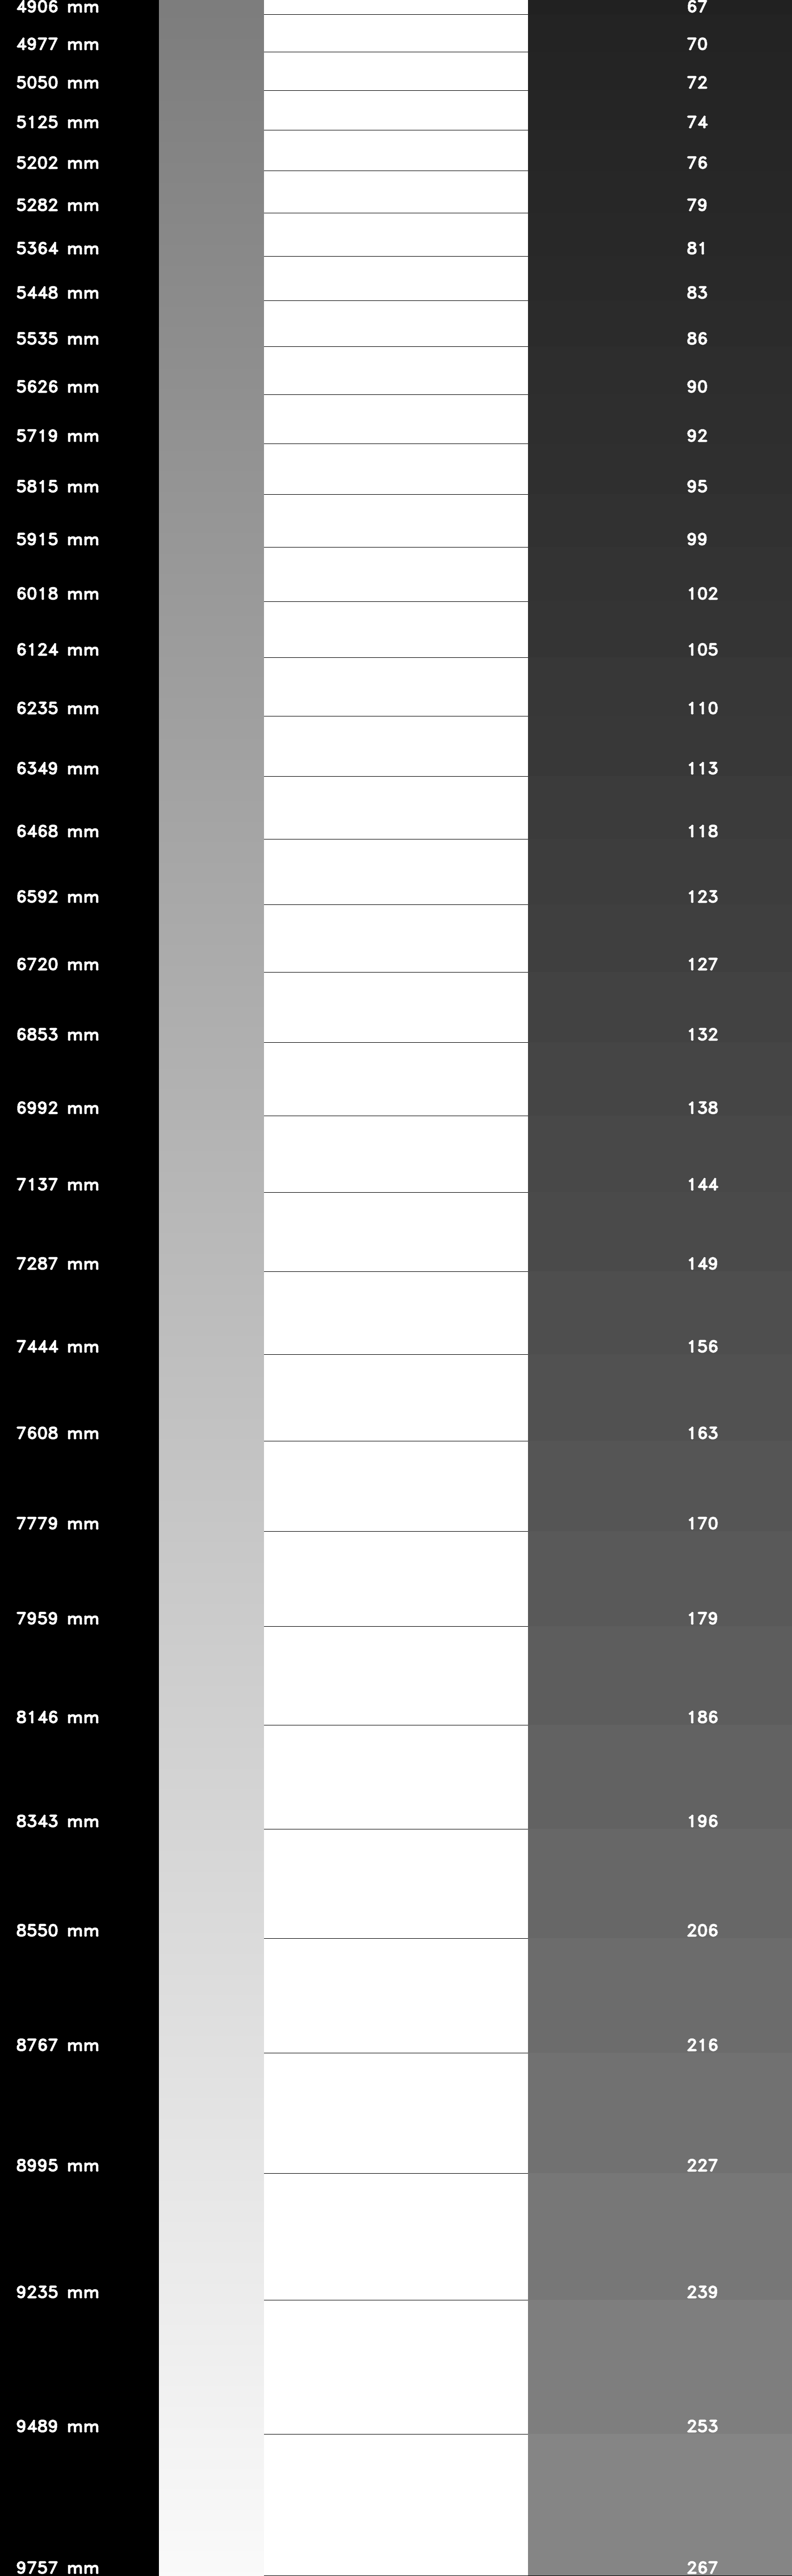
\includegraphics[scale=0.1]{availdepths1.png}
  \caption{Available Depth Values from 4,8 m to 9,8m}
  \label{figure:depths2}
\end{center}
\end{figure}

\begin{figure}[htp]
\begin{center}
  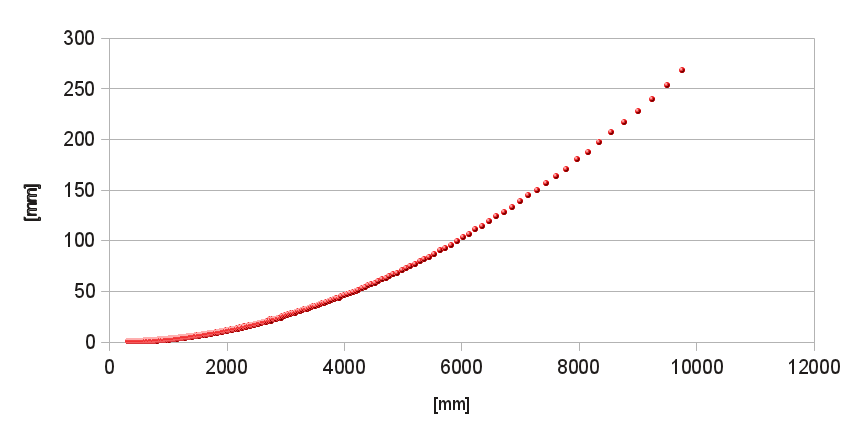
\includegraphics[width=\textwidth]{DifferenceForegoing.png}
  \caption{Missing values in relation to the depth}
  \label{figure:DepthValueDiff}
\end{center}
\end{figure}
